\section{Basic Python structures}
	\subsection{Basic Maths}
You can just start typing maths into Python and it will do it.
		\begin{lstlisting}[language=Python]
1+2\end{lstlisting}
		\begin{verbatim}> 3\end{verbatim}
		
Division in Python 3 gives a decimal answer as you would expect.
		\begin{lstlisting}[language=Python]
5/2\end{lstlisting}
		\begin{verbatim}> 2.5\end{verbatim}
		
		The symbol for power is a double star. A square root can be achieved by raising to the power of 1/2.
		\begin{lstlisting}[language=Python]
2**3\end{lstlisting}
		\begin{verbatim}> 8\end{verbatim}

	\subsection{Variables}\label{types}
		We can store values in variables. You can think of these as ``buckets'' which hold values. You can call variables anything you like as long as it starts with a letter and uses only alphanumeric characters or underscore. In addition it is a very bad idea to use variable names that are reserved keywords elsewhere in Python such as \texttt{print}, \texttt{sum} or \texttt{list}.

The \texttt{print} function prints things to the screen. Here we assign a value to the variable ``a'' using the equals sign and print variable `a''.
		\begin{lstlisting}[language=Python]
a = 6 + 3
print(a)
dead_parrot = "This parrot is no more! He has ceased to be!"
print(dead_parrot)\end{lstlisting}
		\begin{verbatim}> 9
			> This parrot is no more! He has ceased to be!
		\end{verbatim}
		Variables have types. The main types you need to worry about are integers, floats (short for floating point numbers) and strings. Integers are whole numbers, floats are decimals and strings are text. Operations between floats and integers are permitted and the answer will be expressed as a float.
		\begin{lstlisting}[language=Python]
spam = 7
eggs = 0.5
food = spam+eggs
print(food)
\end{lstlisting}
		\begin{verbatim}> 7.5\end{verbatim}	
		Operations between strings and number types are generally not permitted since they make no sense.
		\begin{lstlisting}[language=Python]
song = "I'm a lumberjack and I'm OK" + 1\end{lstlisting}
		\begin{verbatim}> TypeError                                 Traceback (most recent call last)
<ipython-input-47-84d795fdab55> in <module>()
----> 1 "I'm a lumberjack and I'm OK" + 1

TypeError: cannot concatenate 'str' and 'int' objects\end{verbatim}

Strings can be concatenated using the plus symbol.	
		\begin{lstlisting}[language=Python]
line_one = "I'm a lumberjack and I'm OK, "
line_two = "I work all night and I work all day"
song = line_one + line_two
print(song)\end{lstlisting}
		\begin{verbatim}
			> "I'm a lumberjack and I'm OK, I work all night and I work all day"
		\end{verbatim}

	\subsection{Lists}
	Lists are a simple data structure that allow the storage of multiple values. Lists are designated by square brackets. Lists are just another type of variable, so they follow the same variable naming rules.
		\begin{lstlisting}[language=Python]
numberlist = [1, 2, 5]
print(numberlist)\end{lstlisting}
		\begin{verbatim}> [1, 2, 5]\end{verbatim}
		You can fetch a single value from a list by subscripting the list with square brackets. You can fetch multiple values by slicing the list using a colon operator.
		
		\begin{lstlisting}[language=Python]
numberlist = [1, 2, 3, 4, 5, 6, 7]
print(numberlist[4])
print(numberlist[0:3])\end{lstlisting}
		\begin{verbatim}> [5]
			> [1, 2, 3]
		\end{verbatim}
		Notice how the first command returns 5. This is because Python lists (and many things in programming) start counting at zero. This means asking for the zeroth element would return 1.
		The second command returns only three values. This is because the lower bound is inclusive but the upper bound is exclusive (for mostly the same reasons that things start counting at zero not one).

		The append command will add things onto the end of a list. The append command is a method of the list object so acts on the list directly and the result does not need to be assigned to a variable.
		\begin{lstlisting}[language=Python]
numberlist = [1, 2, 5]
numberlist.append(8)
print(numberlist)	\end{lstlisting}
		\begin{verbatim}> [1, 2, 5, 8]\end{verbatim}
		The \texttt{range} function in combination with the \texttt{list} function generates lists that are integer sequences between two specified numbers. The default step size is 1 but this can be changed by supplying the optional ``step'' parameter
\begin{lstlisting}[language=Python]
my_list = list(range(3, 6))
print(my_list)	
my_list = list(range(10, 30, 5))
print(my_list)
\end{lstlisting}
		\begin{verbatim}
> [3, 4, 5]
> [10, 15, 20, 25]\end{verbatim}
		Note how the bounds of the \texttt{range} function work. As for list subscripting, the first value (3) is printed but not the last value (6).

Anywhere you put a value in your code you may use a variable of an appropriate type,
\begin{lstlisting}[language=Python]
lower_bound = 3
eric_the_list = list(range(lower_bound, 11, 2))
print (eric_the_list)
\end{lstlisting}
		\begin{verbatim}
> [3, 5, 7, 9]\end{verbatim}
	\subsection{User input}
		Sometimes it is useful to accept some user input while the program is running and operate on this input. This can be achieved with the input command.
		\begin{lstlisting}[language=Python]
person_name = input("What is your name?")
print("Hello " + person_name)\end{lstlisting}
		\begin{verbatim}
> What is your name?
>> Arthur Pewty
> Hello Arthur Pewty\end{verbatim}
		Note that the input function always interprets the user's input as text. This means that if the input needs to be interpreted as a number then it should be converted explicitly to an integer or float using \texttt{int} or \texttt{float}
		\begin{lstlisting}[language=Python]
user_input_number = float(input("Enter a number: "))
print("Two more than your number is: ", user_input_number+2)\end{lstlisting}
		\begin{verbatim}
> Enter a number: 
>> 40
> Two more than your number is: 42.0\end{verbatim}
\begin{task}Using the \texttt{input}, \texttt{range}, \texttt{int} and \texttt{print} functions, ask the user fo lower and upper bounds and then print a list of integers between the two values.\end{task}
If you want to use only part of a string then strings can be sliced like lists,
		\begin{lstlisting}[language=Python]
name = "The Silly Olympics"
print(name[0:7])
print (name[10:])\end{lstlisting}
\begin{verbatim}
> The Sil
> Olympics\end{verbatim}
If you leave a slice without a second number as in the second example above, the slice will continute until the end of the string. This lets you slice up to the end of the string without having to know exactly how long the string is. This is also true for lists. More about list (and string) slicing can be found in the official Python documentation \url{https://docs.python.org/3/tutorial/introduction.html#lists}.
	\subsection{Flow control}
	For this section we should try using a different IDE. Open a command prompt or terminal and type \texttt{spyder} to open up the Spyder IDE, it may be familiar if you have used MATLAB before. This interactive IDE allows you to edit your code in the left panel and then execute by pressing the run button in the top bar. The ouput is shown in the bottom right window. The top right window is an interactive help window which can provide syntax information for any Python function. There is nothing magic about spyder, you can still run all of this code in a Jupyter notebook (or write it in a text editor and run on the console) but an IDE can be easire to use, especially for bigger projects so see if you prefer it.
		\subsubsection{If statements}
		Programs can only carry out very simple tasks if they do the same thing every time. If programs are able to make decisions based on values supplied to them then this can make them much more powerful. The \texttt{if} statement is the most simple of these flow control tools.
		
		\begin{lstlisting}[language=Python]
penguins = 4

if penguins < 10:
	print(penguins, " is less than 10.")
else:
	print(penguins, " is not less than 10.")
print("This is printed regardless of the number of penguins.")\end{lstlisting}
		\begin{verbatim}
> 4 is less than 10.
> This is printed regardless of the number of penguins.\end{verbatim}	
		Note how the program flow is controlled by the indentation. The \texttt{if} statement  is evaluated and if True then the indented code is run and the else section is skipped. If the \texttt{if} statement  is evaluated and is False, the indented code is skipped and the code beneath the else statement is run. After the \texttt{if}  statement is fully evaluated the program flow returns to the next unindented statement. In this case the last sentence is always printed since it is outside of the \texttt{if} statement. Also the if statement is finished by a colon. This indicates where the question finishes.
		
		If you recall the discussion of types in section \ref{types}, you might have noticed that that the \texttt{print} function seems happy to combine a numeric and string type. This is because \texttt{print} is a special function which converts arguments to strings before printing them. It will only do this if the arguments are separated by a comma as above.
		
		More complex questions can be asked by asking multiple times using the \texttt{elif} statement. The \texttt{elif} statement only executes if the previous statements have been False
		\begin{lstlisting}[language=Python]
num_penguins = 17

if num_penguins < 10:
	print("You have too few penguins.")
elif num_penguins > 10:
	print("That is quite a lot of penguins")
elif num_penguins == 10:
	print("Just the right number of penguins")
else:
	print("This statement should never be printed")\end{lstlisting}
		\begin{verbatim}> That is quite a lot of penguins\end{verbatim}
As with the \texttt{if} statement, syntactically the \texttt{elif} and \texttt{else} statements are finished with a colon (as are all flow control statements).	

It is important to understand the distinction between comparisons and assignment. Notice how on line 1 the assignment operator is one equals sign while on line 7 the comparison operator is two equals signs. The assignment assigns a value to a variable while the comparison operator is asking whether two values are equal.
		\begin{task}Change the above code so that num\_penguins is input by the user when the program is running.\end{task}
		\begin{task}Write a program that takes two numbers from user input, stores them in two variables and then checks whether the numbers are equal. You should display a relevant message depending on whether or not they are equal.\end{task}
		\begin{task} Write a program that asks for the users name, compliments them if it begins with the letter ``P'', insults them if the name is ``Peter'' and if neither or true, repeats the name back again.\end{task}
		\begin{advancedtask}Think about sanitising the user input so that no possible user input can cause an error. Think about users inputting non-alphabetic characters and the case of the characters (PETER should be accepted).\end{advancedtask}


		\subsubsection{For loops}
		\texttt{for} loops are a flow control tool that can be used to repeat a command multiple times by iterating over the members of a sequence.
		\begin{lstlisting}[language=Python]
list_of_numbers = []
for loop_number in range(0, 5):
	list_of_numbers.append(7)
print(list_of_numbers)\end{lstlisting}
		\begin{verbatim}> [7, 7, 7, 7, 7]\end{verbatim}

		\begin{task}What would happen if the \texttt{print} line was also indented?\end{task}
		Each time the for loop is evaluated the next value in the sequence is stored in the ``loop\_number'' variable. This allows you to count
		\begin{lstlisting}[language=Python]
for loop_number in range(3, 7):
	print(loop_number)\end{lstlisting}
\begin{verbatim}
> 3
> 4
> 5
> 6
\end{verbatim}
		This example shows that the number of iterations of the for loop is controlled by the number of elements in the list and not what those elements are, this means you can loop over any arbitrary list, even a list of strings.

Some detail about the \texttt{range} function was omitted earlier. The \texttt{range} function creates a special range object. Previously we have converted this to a list using the \texttt{list} function. However, in these examples by using the range object with the \texttt{for} statement directly, the range object is acting as a generator. This means that for each iteration of the \texttt{for} loop it generates the next number in the sequence. Since only one number at a time is held in memory as opposed to holding the whole list in memory, this increases efficiency when iterating through very large lists.
		\begin{task}Write a program that asks the user for a number \textit{n} and prints the sum of the numbers 1 to \textit{n}.\end{task}
		\begin{task}Modify the previous program so it only sums odd numbers from 1 to n.\end{task}

		\subsubsection{While loops}
		Sometimes it is useful to have a conditional loop. A while loop, repeats a process until a condition is met.
\begin{lstlisting}[language=Python]
secret_number = 4
user_number = 0
user_number = int(input("Guess my number by entering an integer between 1 and 10: "))
while secret_number != user_number:
	print("No, that's not it, guess again.")	
	user_number = int(input("Guess my number by entering an integer between 1 and 10: "))	
print("Yes, that's it.")\end{lstlisting}
		\begin{verbatim}> Guess my number by entering an integer between 1 and 10: 
>> 7
> No, that's not it, guess again.
> Guess my number by entering an integer between 1 and 10:
>> 4
> Yes, that's it.\end{verbatim}
		The comparison operator != checks whether something is not equal. While the two values are not equal the loop will repeat. As soon as they are equal, the loop will exit and the next command will be executed.
\begin{advancedtask}How many integer prime numbers are there under 10,000? Hint: \url{https://en.wikipedia.org/wiki/Generating_primes}\end{advancedtask}

	\subsection{Imports}
		Sometimes we want functions from another package that are not included in the basic Python set of functions. We can import these packages. Here we import the function \texttt{random} from the package \texttt{random} and then use it.
\begin{minipage}{\linewidth}		
\begin{lstlisting}[language=Python]
from random import random
from math import pi

print (random())
print("Pi is: ", pi)\end{lstlisting}
\end{minipage}
		\begin{verbatim}
> 0.29497908252
> Pi is: 3.141592653589793\end{verbatim}
		Packages only need to be imported once per script. This means that imports are usually done at the top of the Python script as the first thing that is done.
		
		The \texttt{random} function prints a random decimal number between 0 and 1.
		\begin{task}Write a for loop that will print out a random number between 0 and 5, 10 times.\end{task}
		\begin{task}Write a for loop that will print out a random integer number between 4 and 10 (including 4 and 10) 5 times.\end{task}
		\begin{task}Program a game of higher or lower. Generate a random integer between 1 and 100. Allow the user to input a guess and tell them if the guess is too high or too low until they guess correctly.\end{task}		
	Some libraries (especially more niche ones) will have to be downloaded and installed separately. Anaconda Python (the Python distribution you have downloaded) is good because it comes with lots of the most popular packages pre-installed.
	\subsection{Subroutines}
			When programs begin to get larger it can be convenient to split the program up into smaller subsections as this makes the logic of the program easier to follow and makes the code easier to maintain. A subroutine, also commonly called a function, is a collection of code that is united under one title that can be ``called'' from elsewhere. Python has many built in functions like \texttt{input}, and \texttt{random}.

In this example we crease a 1 line subroutine,

\begin{minipage}{\paperwidth}
			\begin{lstlisting}[language=Python]
def hungarian_phrasebook():
	print("My hovercraft is full of eels.")

for i in range(0, 2):
	hungarian_phrasebook()\end{lstlisting}
			\begin{verbatim}> My hovercraft is full of eels
			> My hovercraft is full of eels
			\end{verbatim}
\end{minipage}

Lines 1 and 2 define the subroutine but the code in the subroutine does not run until it is called in line 4. When the program runs it first saves the subroutine \texttt{hungarian\_phrasebook} to memory and then begins executing the rest of the code on line 3. 

While this does break up the code somewhat, the subroutine is not very useful since it does exactly the same thing each time it is called. It would be much more useful if it could do different things depending on how we called it. This can be achieved by passing a value to the subroutine called an argument.

			\begin{lstlisting}[language=Python]
def adding_six(input_value):
	print(input_value + 6)

adding_six(3)
adding_six(14)\end{lstlisting}
			\begin{verbatim}> 9
				> 20\end{verbatim}

				Here on line 1 we define the subroutine \texttt{adding\_six} to have the argument \texttt{input\_value}, whenever this subroutine is called it must be given an argument. 

It is a common convention to use a subroutine called \texttt{main}' as the entry point of the code. This means that the code is run starting in \texttt{main} and then splits off into other subroutines. Note that you must remember to call \texttt{main} as seen in line 8. If you don't call \texttt{main} then Python will add all of the subroutines to its memory and then finish without running them!
				
			\begin{lstlisting}[language=Python]
def adding_six(input_value):
	print(input_value + 6)

def main():
	for i in range(0, 2):
		adding_six(i)
		
main()\end{lstlisting}
			\begin{verbatim}> 6
				> 7\end{verbatim}
				
				You can stack as many subroutines as you like, subroutines can call other subroutines and so on. Be careful about how readable your code is though, if you have layers upon layers of subroutines it can be very complex to understand the program flow and there is probably a better way to structure the code. 

				Subroutines don't just have to print values. They can do some processing and then return the value to the parent subroutine using the \texttt{return} function.
			\begin{minipage}{\linewidth}
			\begin{lstlisting}[language=Python]
def adding_six(input_value):
	return input_value + 6

def main():
	number_list = [12, 41, 8, 2]
	
	for i in range(0, len(num_list)):
		number_list[i] = adding_six(number_list[i])
	print(number_list)
			
main()\end{lstlisting}
\end{minipage}

			\begin{verbatim}> [18, 47, 15, 8]\end{verbatim}
			We pass each value of ``number\_list'' into the subroutine \texttt{adding\_six} which adds six and then returns the value to be put back into ``number\_list'', replacing the original value. 

			The distinction between a subroutine and function is not clear and varies depending on which programming language you are talking about. Generally a function is a section of callable code that returns a value while a subroutine does not return a value. Strictly speaking, all subsections of code in Python are functions since they all return a value regardless of whether the return keyword is used. If a function does not explicitly return a value then it returns the number zero to indicate successful completion of the function. For the rest of this tutorial, the words function and subroutine are used interchangeably.

			With larger programs it can be convenient to split subroutines up into entirely different files. For example, if we have some simulation code to run a numerical simulation it would be sensible to split any analysis code off into a separate file. If we have a file called \textit{main.py} and another file called \textit{analysis.py} (in the same directory) containing the subroutine \texttt{do\_analysis} then \textit{main.py} might look like:
\begin{lstlisting}[language=Python]
import analysis

def get_random_number()
	# Chosen by fair dice roll, guaranteed to be random
	random_number = 4
	return random_number
	
def main()
	for counter in range(0, 100):
		test_number = get_random_number()
		analysis.do_analysis(test_number)
			
main()\end{lstlisting}
By importing the file \textit{analysis} in the first line, we can call any functions it contains as if they were in the same file. The syntax is the file name, a period (.) and then the function name.

While this may seem a little complex at first, it is vital to keep code organised as it grows. This will save a lot of time later down the line. 

Also important to organisation is adding comments. By proceeding a line with a hash (\#) we can insert text comments that are ignored by the Python processor. This aids anyone who reads the code in understanding the function of a particular piece of code. Commenting code is another important coding habit.
\begin{task}Do the exercise in section \ref{LJ_excercise}.\end{task}
\begin{advancedtask} Download a list of names from \url{https://merrygoat.github.io/sample_data_3.txt}. Sort these names into alphabetical order. Give each name a value by summing the letter values in the name where A = 1, B = 2... Z = 26. Multiply the name value by the position of the name in the list to get a score for each name. What is the total sum of all of the name scores?\end{advancedtask}

\section{NumPy}
	\subsection{NumPy arrays and vectorisation}
	Computers are fast but not infinitely fast. This means that while trivial calculations can be done without concern for efficiency, more complex calculations such as simulations of thousands of particles often need more care. Python is beautiful and easy to use but it is not the fastest programming language. This means that to do larger calculations we must take some consideration of the efficiency of the programming constructs that we use.

	A very simple way to add 1 to each value in a list would be to step through the list and add 1 to each value.
	\begin{lstlisting}[language=Python]
from time import time

start_time = time()
long_list = range(0, 10000000)

for i in long_list:
	long_list[i] = long_list[i] + 1
end_time = time()

print(end_time-start_time)\end{lstlisting}
	\begin{verbatim}> 2.05770301819\end{verbatim}

	Note the use of the \texttt{time} function in this example. This is a very simple way to assess the speed of code using the system clock. It is not the canonical way to measure performance but like many things in this short tutorial, even if not the best way to do it, it is simple and effective.
	If we think about it then that is fairly impressive, it has been through that loop 10,000,000 times in 2 seconds. But can we make it faster? One key concept in writing speedy code is vectorisation, instead of a loop we want to apply the transformation to every element in the list simultaneously. Let's try that:

	\begin{lstlisting}[language=Python]
short_list = range(0, 5)
print(short_list)
short_list = short_list + 1
print(short_list)\end{lstlisting}

	\begin{verbatim}
> [0, 1, 2, 3, 4]
---------------------------------------------------------------------------
TypeError                                 Traceback (most recent call last)
<ipython-input-9-5d83b7f97176> in <module>()
      3 print short_list
      4 
----> 5 short_list = short_list + 1

TypeError: can only concatenate list (not "int") to list\end{verbatim}

	Basic Python doesn't understand vectorisation. Instead of adding one to each element in the list it is trying to append the number 1 onto the end of the list. This is where NumPy (short for numerical Python) comes in. It is a library that adds data structures and functions suited to mathematical operations. A NumPy array looks like a list but has some subtle differences.

	\begin{lstlisting}[language=Python]
import numpy as np
short_list = [0, 1, 2, 3, 4, 5]
print(short_list)
short_np_array = np.array(short_list)
print(short_np_array)
short_np_array = short_np_array + 1
print(short_np_array)\end{lstlisting}

	\begin{verbatim}
> [0, 1, 2, 3, 4, 5]
> [0 1 2 3 4 5]
> [1 2 3 4 5 6]
	\end{verbatim}

	The NumPy function \texttt{array} generates a NumPy array. It can take a few different types of input but in this case we passed it a regular Python list. This is a type of object like a Python list which holds a series of values. The only difference we see in the output that is printed is that while Python lists have commas separating the values, a NumPy array doesn't. One of the big differences between lists and NumPy arrays underneath is that arrays allow vector operations. This means mathematical operations can be applied to the whole array simultaneously and quickly.

	\begin{lstlisting}[language=Python]
from time import time
import numpy as np

start_time = time()
long_np_array = np.arange(0, 10000000)

long_np_array = long_np_array + 1
end_time = time()

print(end_time-start_time)\end{lstlisting}
	\begin{verbatim}
> 0.0694818496704 \end{verbatim}

	The function \texttt{arange} is a NumPy function that is like \texttt{range} but generates a NumPy array instead of a Python list. Using NumPy arrays instead of lists provides an impressive speedup of nearly 30 times for this simple operation. There are many other useful functions in NumPy and a lot of them make use of the NumPy array as a basic data structure.

\begin{task}Generate a large Python list of data and using a loop take the square root of each element in the list. Now compare the speed when looping through a NumPy array. Finally use the np.sqrt function (Google for how to use it) to vectorise the operation. How much faster is this?\end{task} 

\section{Reading and writing text files}
The amount of data that it is possible to enter by hand is very limited. Often in scientific computing applications the data generated by instruments can be saved to files from where it can be read directly into Python. Some instruments (for example Leica microscopes) may store their data in a proprietary format that is not easy to read. There may by Python libraries which enable you to read the files (this is true for the Leica lif format) or you may have to use some of the manufacturers software to export the data to a simpler format such as a csv or plain text file.
	\subsection{Reading from files}
		The basic way to read in a text file is with the \texttt{open} function. This opens an iterable file object which can be iterated with a for loop to extract each line. For a simple data file with a single column of numbers, one approach might be
		\begin{lstlisting}[language=Python]
data_list = []
input_file = open("example_data_file.txt", 'r')
for line in input_file:
	data_list.append(float(line))
input_file.close()
\end{lstlisting}	
		There are a couple of interesting points here. Firstly, we open the file with the argument \texttt{`r'}. This means read mode, we can read data from the file but not write to it.\\
		Next, data is always read in as a string whether it is characters or digits. This means that to do mathematical operations on numerical data it must implicitly be converted to a float or int type. Be careful though, this is a forceful way of doing things and if the program tries to convert a string into an integer then it will crash. This means that this method is only suitable for input files that we are sure are solely numeric unless some extra checks are added.\\
		The next point is that we close the file object when we are finished reading from it. This is important as Python is connected to the file when the file object is open. If you don't disconnect, then the file link may stay open in the background after Python finishes which may cause problems accessing the file later. Just like a fridge, you need to open the door before taking things in or out but must remember to close the door afterwards.

		Python has a particular style which is not very important for these workshops but is worth discussion in case you want to study the language further. The standard coding style and developments to Python are set out in a series of documents called the Python Enhancement Proposals (PEPs). Some of these documents are very serious and boring proposals while others are poems which set out the recommended style of Python (PEP 20 and 8 are worth a read). In summary, the principle of good Python is readability. The code that you write should be as understandable as possible. Code that follows this principle is called ``Pythonic''. There are certain common Pythonic idioms one of which is seen when handling files. Instead of explicitly opening and closing a file we can use a while loop to do it implicitly
		\begin{lstlisting}[language=Python]
with open("example_data_file.txt", 'r') as input_file:
	for line in input_file:
		data_list = data_list.append(float(line))
\end{lstlisting}	
This way the file is opened at the \texttt{with} statement and kept open for all of the indented statements. It doesn't have to be explicitly closed as it is done automatically when the \texttt{with} statement is left.

At the end of the day it is up to you. While there are some commonly adopted standards, you can do whatever you think makes your code the most readable. Your style will certainly change and your code will become more beautiful as you learn more.

\begin{task}Download a sample data file from: \url{https://merrygoat.github.io/sample_data_1.txt}. Read the data in to Python and print the numbers to screen.\end{task}

	\subsection{Writing to files}
		Writing to files is similar to reading from files but this time we have to open the file in write mode
		\begin{lstlisting}[language=Python]
my_calculated_data = [4, 5, 6, 7]
with open("example_data_file.txt", 'w') as output_file:
	for number in range(0, len(my_calculated_data)):
		output_file.write(str(my_calculated_data[number]) + "\n")
\end{lstlisting}	
	Here the \texttt{`w'} in the \texttt{open} function is opening ``example\_data\_file.txt'' in write mode. This means that if the file does not exist on disk it will be created and if it already exists the file will be overwritten. If you want to write to a file that already exists then you need to open in write append mode, \texttt{`a'}.
Note again that file operations are done with strings so numbers have to be explicitly converted before writing to the file. But what is the \texttt{``\textbackslash{}n''} at the end? This is the special character for a new line. This ensures that each of our numbers will be printed to a new line.

\begin{task}Read in the dataset from the last task, multiply each number by two and save it to a new text file.\end{task}

Reading and writing to files directly like this is good if the file you want to read or write requires a specific or complex format. These methods can also write combinations of numbers and strings which can be useful. However, most of the time our data analysis will just be done on grids of numbers. For this there is an easier way with NumPy.

	\subsection{NumPy loadtxt}
		Most likely whatever experiment or simulation we have done will have already written data to a file that can be read. Most simulations and some experimental equipment will allow you to output your data as a plain text file. There are many functions from different libraries that allow file reading but for simple text files of numbers \texttt{loadtxt} is easy to use.
		\begin{lstlisting}[language=Python]
import matplotlib.pyplot as plt
x_data, y_data = np.loadtxt("example_input_data.txt", skiprows=1, unpack=True)
plt.plot(x_data, y_data)
plt.show()\end{lstlisting}

Here we use Matplotlib to plot the data on a graph, the details are not important right now, we will look at it in more detail in section \ref{matplotlib}.

\texttt{loadtxt} is a fairly basic way of reading in data files. It will only read in grids of data and will struggle if there are data points missing. Notice how we use the skipline command to skip the title line in the file. Try without the skipline parameter and see what happens. The unpack parameter is also important, this reads the first column into the first variable and the second column into the second variable we specified. Without the unpack parameter the data would be read into the first variable in as 2 column array. Again, try the code without the unpack parameter and see what happens.

Since \texttt{loadtxt} reads the data into a NumPy array it accepts only numbers as input. If you need to read in a mixture of text and numbers this is probably better done with a Python list and a basic file read loop. If you have numerical data with a more complex layout such as missing values then \texttt{genfromtxt} is a more complex but flexible file reading function.

\begin{task}Download a sample data file from \url{https://merrygoat.github.io/sample_data_2.txt}. Read in this data using \texttt{loadtxt} and print it to the screen.\end{task}

	\subsection{NumPy savetxt}
		In the same way as before, if you just have a simple NumPy array of data, you can quickly save to a text file with NumPy \texttt{savetxt},
		\begin{lstlisting}[language=Python]
my_clever_data = np.array([[2, 3], [4, 5], [6, 7]])

np.savetxt("output.txt", my_clever_data)\end{lstlisting}

\begin{task}Using the input from the previous exercise, read in the data using \texttt{loadtxt}, multiply the values in the second column by 4 and print to a file using \texttt{savetxt}. Check the \texttt{savetxt} documentation for how to save a title line before the data.\end{task}

\section{Matplotlib}\label{matplotlib}
	\subsection{Histograms}
		There is a very powerful package called Matplotlib that provides functions for plotting graphs. Matplotlib is used across academia as well as elsewhere for producing publication quality figures. At first it might seem like a lot of effort to learn an entirely new script based method for plotting compared to something like Excel but it is worth it. Matplotlib graphs look much better than Excel ones, they are much more customisable and more powerful. You can also output files in vector format which is required for submission to most journals. In addition, once you have a nice set of templates set up you can use them all through your academic career, slightly modifying them to suit whatever data you have.
		\begin{lstlisting}[language=Python]
%matplotlib inline
import matplotlib.pyplot as plt

listofnumbers=[0.2, 0.3, 0.4, 1.2, 1.7, 1.9, 2.2, 2.5, 3.1, 3.4, 4.6, 5.1, 5.6, 6.0, 7.4, 7.4, 7.6]
plt.hist(listofnumbers, bins=[0, 1, 2, 3, 4, 5, 6, 7])
plt.show()\end{lstlisting}
		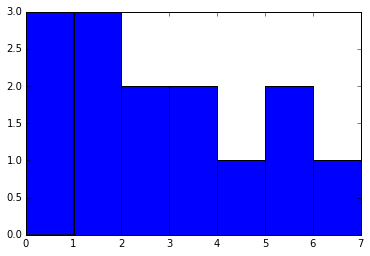
\includegraphics[scale=0.7]{images/histogram}

		First we import the Matplotlib library, then the command \texttt{\%matplotlib inline} tells Jupyter Notebook to plot the graphs in the workbook rather than opening them in another window. You only need this command once per session so it is common to put it at the top with the \texttt{import} commands. Then we generate a list of numbers and plot them as a histogram.
		\begin{task}What does the bins argument do? What happens if you leave it out entirely?\end{task}
		\begin{task}Generate 1000 random numbers between 0 and 10 using a for loop and append them to a list. Plot a histogram of this list.\end{task}
		\begin{task}Complete the exercise in section \ref{pi_exercise}.\end{task}

	\subsection{Line Plots}
		Line plots are made in a similar way to histograms,
		\begin{lstlisting}[language=Python]
x_data=[2011, 2012, 2013, 2014, 2015, 2016, 2017]
y_data=[58, 68, 65, 71, 78, 81, 78 ]
plt.plot(x_data, y_data, linestyle = "-", marker = "x", markersize=10, linewidth=2)
plt.title("Confuse-a-cat sucess rate")
plt.xlabel("Year")
plt.ylabel("Percentage of cats confused")
plt.savefig("confuseacat.pdf")
plt.show()\end{lstlisting}
		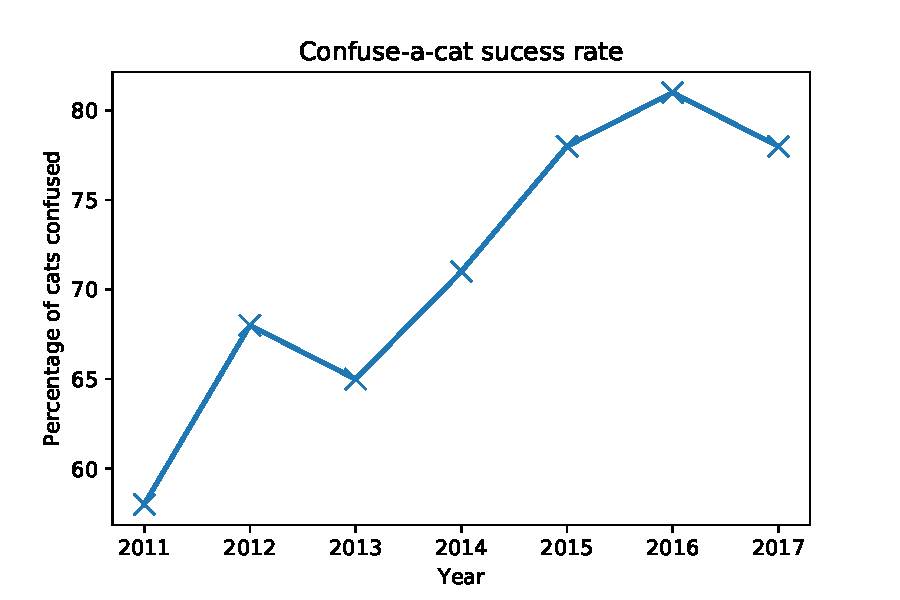
\includegraphics[scale=0.75]{images/confuseacat}

You can read the full specification for the plot function online: \url{https://matplotlib.org/api/pyplot_api.html#matplotlib.pyplot.plot}. This gives details about the marker and line types and other things like how to change the line and marker colours.
\begin{task}Adjust the axis range of the graph so it shows the percentage axis from 0 to 100. Google something like ``matplotlib axis range example'' to find the correct syntax.\end{task}
Googling things is a very important skill that needs practice. There is always more than one way to do a simple task like this so have a look at a few different ones and see what works best. Beware that some of the examples you will find are hard to understand, inefficient or just wrong! You need to distinguish between these and pick out the right commands for your task.
\begin{task}Using sample\_data2 from \url{https://merrygoat.github.io/sample_data_2.txt}, read in this data and plot as a scatter plot.\end{task}

\section{Fitting Data}
	Fitting data is easy in something like Origin but this is a poor approach if you have to fit 100 datasets. As with everything in programming, it takes a little time to set up a script but if you have to run it 100 times then you can save a lot of time.

The first part is to define a function that describes your fit. It should have the independent variable as the first argument and the adjustable variables afterwards,
\begin{lstlisting}[language=Python]
def linear_function(x, m, c):
	return m * x + c
\end{lstlisting}

Then once you have some data you can use the \texttt{curve\_fit} function from scipy.optimize to find the optimal fitting parameters.
\begin{lstlisting}[language=Python]
x_data = [1, 2, 3, 4, 5, 6]
y_data = [3.2, 4.9, 7.1, 8.7, 10.9, 13.2]

popt, pcov = curve_fit(linear_function, x_data, y_data)
\end{lstlisting}
``popt'' stores the optimal fitting parameters while ``pconv'' stores the covariance of the fit.
Now to plot this fit we have to generate some x-values and determine the corresponding y-values using the parameters we have determined.
\begin{lstlisting}[language=Python]
x_fit = np.arange(1, 6, 0.01)
y_fit = linear_function(x_fit, popt[0], popt[1])
\end{lstlisting}
\texttt{arange} is generating an array of x-values from 1 to 6 at 0.01 intervals. The y-values are then found by putting the x-values and optimised fitting parameters into the fitting function. After this we can plot the original data as points and the fit as a line. Putting all of this together gives us

\begin{lstlisting}[language=Python]
import matplotlib.pyplot as plt
import numpy as np
from scipy.optimize import curve_fit
%matplotlib inline

def linear_function(x, m, c):
    return m * x + c

# Generate the data
x_data = [1, 2, 3, 4, 5, 6]
y_data = [3.2, 4.9, 7.1, 8.7, 10.9, 13.2]

# Determine the fit parameters
popt, pcov = curve_fit(linear_function, x_data, y_data)

# Generate fit data for plotting
x_fit = np.arange(1, 6, 0.01)
y_fit = linear_function(x_fit, popt[0], popt[1])

# Plot original data and the fit
plt.plot(x_data, y_data, marker="x", markersize=10, linewidth=0)
plt.plot(x_fit, y_fit, linewidth=2)
plt.xlabel("Time spent learning Python (hours)", fontsize=12)
plt.ylabel("Love of Python (arbitrary units)", fontsize=12)
plt.show()
\end{lstlisting}
\begin{task}Using the data from sample\_data2 (\url{https://merrygoat.github.io/sample_data_2.txt}) fit and plot a log curve to the data. What are the coefficients?\end{task}

\section{Exercises}
	\subsection{Lennard-Jones potential}\label{LJ_excercise}
		The Lennard-Jones potential is a model potential which is used to describe the pair interaction between two atoms as a function of their separation,
\begin{equation}u_{LJ}(r) = 4\epsilon \left [ \left (\frac{\sigma}{r} \right )^{12}- \left (\frac{\sigma}{r} \right )^{6} \right ]\end{equation}
	where $r$ is the interparticle separation, $\epsilon$ is the well depth and $\sigma$ is the separation where the interaction strength zero. For atomic argon, $\sigma = 3.4*^{-10} \mathrm{m}$ and $\epsilon= 1.65*10^{-21} \mathrm{J}$.
	
\textbf{Write a function which returns the interaction energy of two argon atoms as a function of their separation.}

	\subsection{Calculation of pi}\label{pi_exercise}
		Some processes can be modelled using random numbers. One of the simplest examples of this is finding the value of pi. Pi is the ratio of a circle's radius to its circumference. Equivalently we can say that pi is the ratio of the area of an inscribed circle of a square to the area of the square. This is illustrared in Fig. \ref{fig:picircle}. 
	\begin{figure}[h]
		\centering
		\includegraphics[scale=0.4]{images/pi}
		\caption{The blue circle is inscribed in the black dashed square.}
		\label{fig:picircle}
	\end{figure}

	If we pick a series of random points inside the square then some will fall inside the circle and some will fall outside. The ratio of these two quantities will tell us the relative areas of the two shapes. From this we can calculate pi.

	How can we tell if a random point is inside the circle or not? The Pythagorean theorem tells us the hypotenuse of a right angled triangle. For a circle radius 1 we know that a point is inside the circle if:

	\begin{equation}
	\sqrt{a^2+b^2} <= 1,
	\end{equation}

	where $a$ and $b$ are the side lengths of the triangle. Since the circle is symmetric, we don't need the whole thing, just a quarter will do. This makes the generation of random numbers easier since we can generate numbers between 0 and 1 to put random coordinates inside a box of side length 1. This scheme is shown in Fig. \ref{fig:piarc}

	\begin{figure}[h]
		\centering
		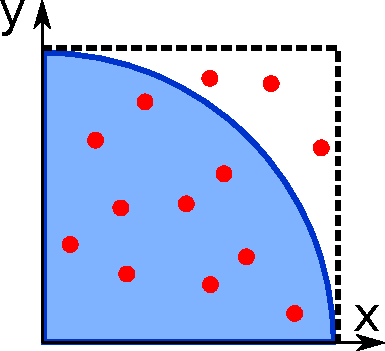
\includegraphics[scale=0.6]{images/piarc}
		\caption{If we pick random points on the figure some will fall outside the circle and some inside. The ratio of the two allows us to find pi.}
		\label{fig:piarc}
	\end{figure}

	\textbf{Using all of the above techniques, calculate pi using random numbers. Try using 100, 1000, 10,000 or more random samples, how does this affect the error? If you calculate pi 1000 times and plot a histogram of these values, what sort of distribution would you expect the values to follow and why? What is the nature of the relationship between number of samples and distribution width?}
	If you find this task too hard, there are some hints in Appendix \ref{app:pi_hints}. Try not to look at them unless you are really stuck. Learning (of programming in particular) works much better if you got through the process of problem solving rather than just reading the answer. The hints in Appendix \ref{app:pi_hints} are graded in terms of difficulty. The first hint gives you a little help and the subsequent hints more help.